\chapter{Задание}

\textbf{Цель работы}: построение доверительных интервалов для математического ожидания и дисперсии нормальной случайной величины.

\begin{enumerate}
	\item Для выборки объема $n$ из нормальной генеральной совокупности $X$ реализовать в виде программы на ЭВМ
		\begin{enumerate}
			\item вычисление точечных оценок $\hat\mu(\vec x_{n})$ и $S^2(\vec x_{n})$ математического ожидания M$X$ и дисперсии D$X$ соответственно;
			\item вычисление нижней и верхней границ $\underline{\mu}(\vec x_{n})$, $\overline{\mu}(\vec x_{n})$ для \newline$\gamma$-доверительного интервала для математического ожидания M$X$;
			\item вычисление нижней и верхней границ $\underline{\sigma}^2(\vec x_{n})$, $\overline{\sigma}^2(\vec x_{n})$ для \newline$\gamma$-доверительного интервала для дисперсии $DX$;
		\end{enumerate}
	\item вычислить $\hat\mu$ и $S^2$ для выборки из индивидуального варианта;
	\item для заданного пользователем уровня доверия $\gamma$ и $N$ --- объема выборки из индивидуального варианта:
		\begin{enumerate}
			\item на координатной плоскости $Oyn$ построить прямую $y = \hat\mu(\vec x_{N})$, также графики функций $y = \hat\mu(\vec x_{n})$, $y = \underline{\mu}(\vec x_{n})$ и $y = \overline{\mu}(\vec x_{n})$ как функций объема $n$ выборки, где $n$ изменяется от 1 до $N$;
			\item на другой координатной плоскости $Ozn$ построить прямую \newline$z = S^2(\vec x_{N})$, также графики функций $z = S^2(\vec x_{n})$, $z = \underline{\sigma}^2(\vec x_{n})$ и $z = \overline{\sigma}^2(\vec x_{n})$ как функций объема $n$ выборки, где $n$ изменяется от 1 до $N$.
		\end{enumerate}
\end{enumerate}

\chapter{Теоретическая часть}

\section{Определение $\gamma$-доверительного интервала для значения параметра распределения случайной величины}

Пусть $X$ --- случайная величина, закон распределения которой зависит от вектора $\vec \theta = (\theta_{1}, ..., \theta_{r})$ неизвестных параметров. Будем считать, что $r = 1$, т. е. $\vec \theta = (\theta_{1}) = (\theta)$.

\underline{Опр.} Интервальной оценкой параметра $\theta$ уровня $\gamma$ ($\gamma$-интервальной оценкой) называют пару статистик $\underline{\theta}(\vec X)$ и $\overline{\theta}(\vec X)$ таких, что
\begin{equation}
	P\{\theta \in (\underline{\theta}(\vec X), \overline{\theta}(\vec X))\} = \gamma, \gamma \in (0;1).
\end{equation}

\underline{Опр.} $\gamma$-доверительным интервалом (доверительным интервалом уровня $\gamma$) для параметра $\theta$ называют реализацию (выборочное значение) интервальной оценкой уровня $\gamma$ для этого параметра, т.е. интервал $(\underline{\theta}(\vec x), \overline{\theta}(\vec x))$ с детерминированными границами.

\section{Формулы для вычисления границ \newline$\gamma$-доверительного интервала для математического ожидания и дисперсии нормальной случайной величины}

Пусть $N(\mu, \sigma^2)$ --- общий вид закона распределения генеральной совокупности $X$. $\mu$, $\sigma^2$ --- неизвестны. 

Границы $\gamma$-доверительного интервала для математического ожидания нормальной случайной величины:
\begin{equation}
	\underline{\mu}(\vec X) = \overline{X} - \frac{S(\vec X)t^{(n - 1)}_{\frac{1 + \gamma}{2}}}{\sqrt{n}},
\end{equation}
\begin{equation}
	\overline{\mu}(\vec X) = \overline{X} + \frac{S(\vec X)t^{(n - 1)}_{\frac{1 + \gamma}{2}}}{\sqrt{n}},
\end{equation}
где $\overline{X} = \frac{1}{n} \sum_{i=1}^n X_i$; $S(\vec X) = \sqrt{\frac{1}{n-1} \sum_{i=1}^n (X_i - \overline X)^2}$; $t^{(n - 1)}_{\frac{1 + \gamma}{2}}$ --- квантиль уровня $\frac{1 + \gamma}{2}$ распределения Стьюдента с $n - 1$ степенями свободы; $n$ --- объем выборки.

Границы $\gamma$-доверительного интервала для дисперсии нормальной случайной величины:

\begin{equation}
	\underline{\sigma}^2(\vec X) = \frac{(n - 1)S^2(\vec X)}{h^{(n - 1)}_{\frac{1 + \gamma}{2}}},
\end{equation}
\begin{equation}
	\overline{\sigma}^2(\vec X) = \frac{(n - 1)S^2(\vec X)}{h^{(n - 1)}_{\frac{1 - \gamma}{2}}},
\end{equation}
где $n$ --- объем выборки; $S^2(\vec X) = \frac{1}{n-1} \sum_{i=1}^n (X_i - \overline X)^2$; $h^{(n - 1)}_{\frac{1 + \gamma}{2}}$, $h^{(n - 1)}_{\frac{1 - \gamma}{2}}$ --- квантили уровня $\frac{1 + \gamma}{2}$ и $\frac{1 - \gamma}{2}$ соответственно распределения $\chi^2(n - 1)$.

\chapter{Практическая часть}

\section{Текст программы}

\begin{lstlisting}[style={Matlab}]
function lab_02
    X = [14.90,14.40,13.56,15.55,13.97,16.33,14.37,13.46,15.51,14.69,...
         13.41,14.24,15.65,14.54,13.55,13.15,14.32,15.04,13.27,14.60,...
         13.83,13.93,14.11,14.15,15.48,15.96,14.46,13.87,13.67,15.30,...
         13.95,16.08,18.25,14.93,15.37,14.38,15.56,13.92,14.23,12.80,...
         13.16,13.89,14.24,13.90,12.82,13.20,13.89,13.50,13.44,16.13,...
         14.68,15.27,13.35,13.62,16.16,16.46,13.83,14.13,15.68,15.22,...
         12.59,12.94,13.09,16.54,14.61,14.63,14.17,13.34,16.74,16.30,...
         13.74,15.02,14.96,15.87,16.03,12.87,14.32,14.48,14.57,14.43,...
         12.61,14.52,15.29,12.07,14.58,11.74,14.97,14.31,12.94,12.82,...
         14.13,14.48,12.25,14.39,15.08,12.87,14.25,15.12,15.35,12.27,...
         14.43,13.85,13.16,16.77,14.47,14.89,14.95,14.55,12.80,15.26,...
         13.32,14.92,13.44,13.48,12.81,15.01,13.19,14.68,14.44,14.89];
    n = length(X);

    mu = sum(X) / n;
    S2 = sum((X-mu).^2) / (n - 1);
    fprintf("Выборочное среднее = %.4f\n", mu);
    fprintf("Исправленная выборочная дисперсия = %.4f\n", S2);
    
    gamma = 0.9;
    mu_bottom = get_mu_bottom(gamma, n, mu, S2);
    mu_top = get_mu_top(gamma, n, mu, S2);
    fprintf("\n%.1f-доверительный интервал для математического ожидания: (%.4f, %.4f)\n", gamma, mu_bottom, mu_top);
    
    S2_bottom = get_S2_bottom(gamma, n, S2);
    S2_top = get_S2_top(gamma, n, S2);
    fprintf("\n%.1f-доверительный интервал для дисперсии: (%.4f, %.4f)\n", gamma, S2_bottom, S2_top);

    mu_arr = zeros(1, n);
    S2_arr = zeros(1, n);
    mu_bottom_arr = zeros(1, n);
    mu_top_arr = zeros(1, n);
    S2_bottom_arr = zeros(1, n);
    S2_top_arr = zeros(1, n);

    for i = 1 : n
      mu_arr(i) = sum(X(1:i)) / i;
      
      if i == 1
        S2_arr(i) = 0;
      else
        S2_arr(i) = sum((X(1:i)-mu_arr(i)).^2) / (i - 1);
      end
      
      mu_bottom_arr(i) = get_mu_bottom(gamma, i, mu_arr(i), S2_arr(i));
      mu_top_arr(i) = get_mu_top(gamma, i, mu_arr(i), S2_arr(i));
      
      S2_bottom_arr(i) = get_S2_bottom(gamma, i, S2_arr(i));
      S2_top_arr(i) = get_S2_top(gamma, i, S2_arr(i));
    end
    
    clf;
    plot(1:n, zeros(1, n) + mu, "k");
    hold on;
    plot(1:n, mu_arr, "r");
    plot(1:n, mu_bottom_arr, "g");
    plot(1:n, mu_top_arr, "b");
    xlabel("n");
    ylabel("y");
    l = legend('y = \mu^{\^}(x_N)', 'y = \mu^{\^}(x_n)', 'y = \mu_{bottom}(x_n)', 'y = \mu_{top}(x_n)');
    set(l, "interpreter", "tex");
    grid on;
    figure;
    plot(1:n, zeros(1, n) + S2, "k");
    hold on;
    plot(1:n, S2_arr, "r");
    plot(1:n, S2_bottom_arr, "g");
    plot(1:n, S2_top_arr, "b");
    xlabel("n");
    ylabel("z");
    l = legend('z = S^2(x_N)', 'z = S^2(x_n)', 'z = \sigma^2_{bottom}(x_n)', 'z = \sigma^2_{top}(x_n)');
    set(l, "interpreter", "tex");
    grid on;
endfunction

function mu_bottom = get_mu_bottom(gamma, n, mu, S2)
    t = tinv((1 + gamma)/2, n - 1);
    mu_bottom = mu - sqrt(S2) * t / sqrt(n);
end

function mu_top = get_mu_top(gamma, n, mu, S2)
    t = tinv((1 + gamma)/2, n - 1);
    mu_top = mu + sqrt(S2) * t / sqrt(n);
end

function S2_bottom = get_S2_bottom(gamma, n, S2)
    h_bottom = chi2inv((1 + gamma)/2, n - 1);
    S2_bottom = (n - 1) * S2 / h_bottom;
end

function S2_top = get_S2_top(gamma, n, S2)
    h_top = chi2inv((1 - gamma)/2, n - 1);
    S2_top = (n - 1) * S2 / h_top;
end
\end{lstlisting}

\section{Результаты расчетов и графики для выборки из индивидуального варианта}

\begin{lstlisting}[style={Matlab}]
Выборочное среднее = 14.3492
Исправленная выборочная дисперсия = 1.2776

0.9-доверительный интервал для математического ожидания:
(14.1781, 14.5202)

0.9-доверительный интервал для дисперсии: (1.0452, 1.6036)
\end{lstlisting}

\begin{figure}[H]
	\begin{center}
		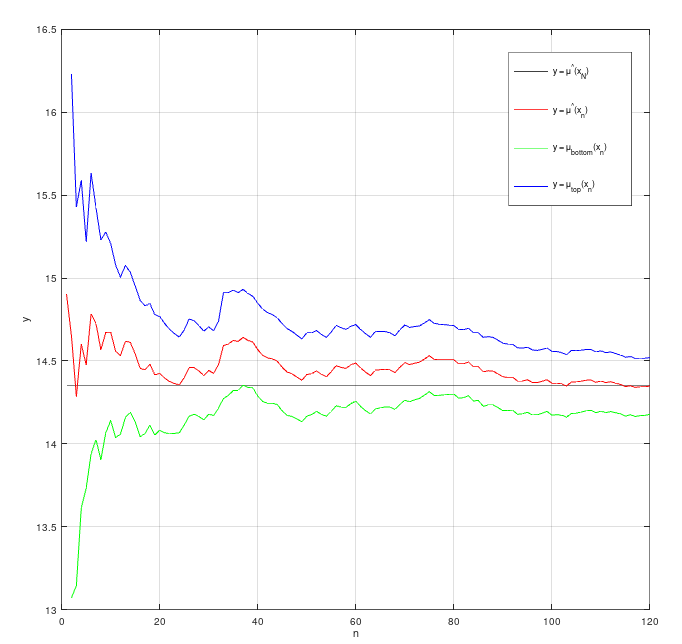
\includegraphics[scale=0.7]{img/Oyn.png}
	\end{center}
	\captionsetup{justification=centering}
	\caption{Прямая $y = \hat\mu(\vec x_{N})$ и графики функций $y = \hat\mu(\vec x_{n})$, $y = \underline{\mu}(\vec x_{n})$ и $y = \overline{\mu}(\vec x_{n})$ как функций объема $n$ выборки, где $n$ изменяется от 1 до $N$}
	\label{img:bar}
\end{figure}

\begin{figure}[H]
	\begin{center}
		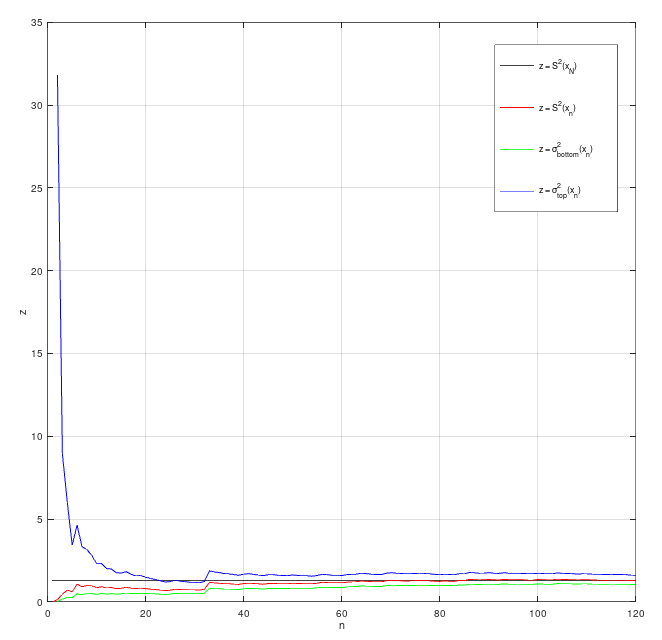
\includegraphics[scale=0.6]{img/Ozn.png}
	\end{center}
	\captionsetup{justification=centering}
	\caption{Прямая $z = S^2(\vec x_{N})$ и графики функций $z = S^2(\vec x_{n})$, $z = \underline{\sigma}^2(\vec x_{n})$ и $z = \overline{\sigma}^2(\vec x_{n})$ как функций объема $n$ выборки, где $n$ изменяется от 1 до $N$}
	\label{img:graph}
\end{figure}